\section{Discussion}
\label{s:discussion}

\begin{table*}[t]
  \centering
  \begin{center}
    \begin{tabularx}{1\textwidth}{c|c|c|c|c|c}
    \toprule
    \multicolumn{6}{c} {$W$: number of words, $T$: number of tags,
    $L$: number of links} \\
    \midrule
      Methods & Features & Complexity &
      Efficiency & Effectiveness & Deployment \\
      \hline
      Najork ~\cite{najork2005system} & words, links, tags 
      & $O(W^2 + L^2 + T^2)$ & low & low & User \\
      Term \& Link Diff ~\cite{wu2005cloaking} & words and links & $O(W^2 + L^2)$
      & low & medium  & Server  \\
      Wu \& Davison ~\cite{wu2006detecting} & words, links & $O(W^2 + L^2)$ & 
      low & medium &  Server \\
      CloakingScore ~\cite{chellapilla2006improving} & words & $O(W^2)$ &
      low & medium & Server  \\
%      Click-Through ~\cite{wang2006detecting} & click-through  & 
%      $O(W^2 + L^2 + T^2)$ & high & low & Server  \\
      TagDiff ~\cite{lin2009detection} & tags  & $O(T^2)$  & medium &
      medium &  Server  \\
      Cloaker and Dagger ~\cite{wang2011cloak} & words, tags  &  $O(W +
      T^2)$ & medium & high & Server \\
      Hybrid Detection ~\cite{deng2013uncovering} & words, links, tags &
      $O(W + L^2 + T^2)$ & medium & high & Server \\
      SWM & words, tags & $O(W + T)$ & high & high & Server and User \\
      \bottomrule
    \end{tabularx}
  \end{center}
  \caption{Comparison of cloaking detection methods}
  \label{comparison}
\end{table*}

In this section, we first compare our work with previous cloaking detection
works, then discuss two kinds of deployment of simhash-based cloaking
detection system: server-based and crowdsoucing-based. We analyze the attack models
and robustness of crowdsourcing model.

\subsection{Efficiency Comparison}
\label{ss:efficiency}
Previous cloaking detection approaches use different feature sets from a website,
and the latest work ~\cite{wang2011cloak} use text features, dom features and
search snippet to detect cloaking. Comparing with their model, we achieve
similar precision and recall (transformed from FPR and TPR). However, a great
advantage of our work over past approaches is that, our algorithm is
efficient and clean: requires only single pass of website to get fuzzy signature and then
compare fuzzy signatures instead of the original document. This feature 
not only saves time and make cloaking detection scalable, 
but also enables data collection to be deployed at user side for crowdsourcing.

~\autoref{comparison} compares past cloaking detection approaches. Our approach
use the content that contains most information (entropy), and is more efficient
compared to past approaches. Regarding text simhash and DOM simhash generation,
we implement a browser plugin and it introduces little overhead to browsing
session. Besides, in order to further reduce overhead to browser, simhash
computation can be triggered under some circumstances. For example, compute
simhash only when advertisements are visited (url contains specific string), and
set computation probability to $p = \frac{1}{100}$ to further reduce overhead.

%Compared with past approaches, we achiev
%While we can achieve similar false positve rate and true positive rate compared
%to past approaches, we argue that, our approach is much more efficient than past
%approaches and is light-weight enough to be deployed on user browser.
%\XXX{Table} is a comparison of time complexity and number of rounds that the
%documents need to be processed (each time they get smaller amount of document,
%though). Let $N$ denote the number of total urls collected, $M$ denoete the
%number of cloaking websites. The time complexity is \XXX{Plot}.





\subsection{Server-based Deployment}
In server-based cloaking detection system,
we first collect targeted search words includes commecial terms, cloaking oriented terms and hot trend words.
Using these search words, the system retrieves the search results from the search engines for seven times.
First, the system disguises as normal user by using normal user agent. Next, the
system disguises as Google crawler by using the Google Agent and visit landing
pages obtained from the first visit. With this data that
is crawled from Google view, the system uses the simhash method to model the websites.  
The system compares simhash value from user view and
website model learned from Google view. From the comparsion result, the system judges if the website is cloaking
or not. 
Server based cloaking detection system has pros and cons. The deployment of server based cloaking dectetion system
is pratical and could be deployed
easily. The tradeoff of easy deployment is inefficient in IP cloaking detection. Usually, the servers IP addresses
are in a range,  scammers could find this range and serve benign content to crawlers. One solution is buying numerous IP addresses
from ISP providers and distributing IP addresses as similar to real user distribution. This increases cloaking detection cost. In
addition, distributing IP addresses as users is hard. Further, server-based cloaking detection system is infeasiable
to detect cloaking in search engine marketing(SEM). As we mentioned, using the crawlers to visit websites in SEM field
increases the advertisement cost of websites. Moreover, different websites has
different changing periods. For example, {\it www.yahoo.com} 
updates fast, but {\it www.apple.com} is relatively slow. Identifying different 
crawling periods for different websites is difficult. 

\subsection{Crowdsourcing-based Deployment}
Crowdsourcing cloaking detection system includes user-side and server-side component. In user side, users needs to install the cloaking
detection extension in their browers. While users click search results and view
websites, the extension computes the simhash value based on 
website content and layouts. After calculation, extension packs URL and simhash
value and sends to server. Server passively receives $(URL, simhash value)$
pairs from users. Server also utilizes crawlers to extract content several times
from this URL from search engine view (crawler uses Google bot agents).
Server uses these extracted content to model the website. Through comparing
$(URL, simhash value)$ pair from users and crawler view,
server could decide if the website is cloaking or not. As mentioned in
~\autoref{s:measurement}, incentives behind cloaking includes domain parking
~\cite{vissers2015parking} (suspicious) and
malware distribution. Based on cloaking
detection result, server categorizes cloaking and update blacklists in browsers' extensions.
Updating blacklists and warning users phishing and
malware downloading is users incentive to install our extension.

~\autoref{fig:workflow} explains the proposed crowdsourcing-based cloaking detection framework. 
Next, We discuss the pros and cons for this approach. The first advantage is privacy. Instead of solicting
website content from users, the system solicited a 64 bits simhash value from users. 
From this 64 bits value, system couldn't do reverse engineering to
get original content. In addition, the system could intergrate with 
RAPPOR~\cite{erlingsson2014rappor}, which protect the privacy of URL.
Because the workflow is similar to safe browsing API ~\cite{rajab2013camp} , we argue that this can be easily
extended in current framework, the only different is that (URL, simhash value)
pair is processed through RAPPOR to achieve anonymity.

In addition, the crowdsouring deployment introduces low traffic. Browsers only send a 64 bits value for
each URL. This won't jam traffic. Further, the crowdsoucing deployment 
wouldn't affect the model of SEM. Each click on advertisements of search engines is
from real users instead of crawlers. Advertisers don't need to pay extra money for cloaking detection. 


%Employ RAPPOR~\cite{erlingsson2014rappor} to provide user privacy gurantee.
%
%pros: 	1.privacy 2.Low traffic. 3.SEM 4.Distributed computation 
%5. Remove the need to do redirect cloaking detection, leveraging the feature
%that the end goal of attackers is to reach user
%6. could decide crawl period passively based on user clicks, data received are
%based on real user’s clicks, say, website traffic
%
%cons: user incentives. 
%Solution: Plugin to detect suspicious websites. API


\begin{figure}[t]
  \centering
  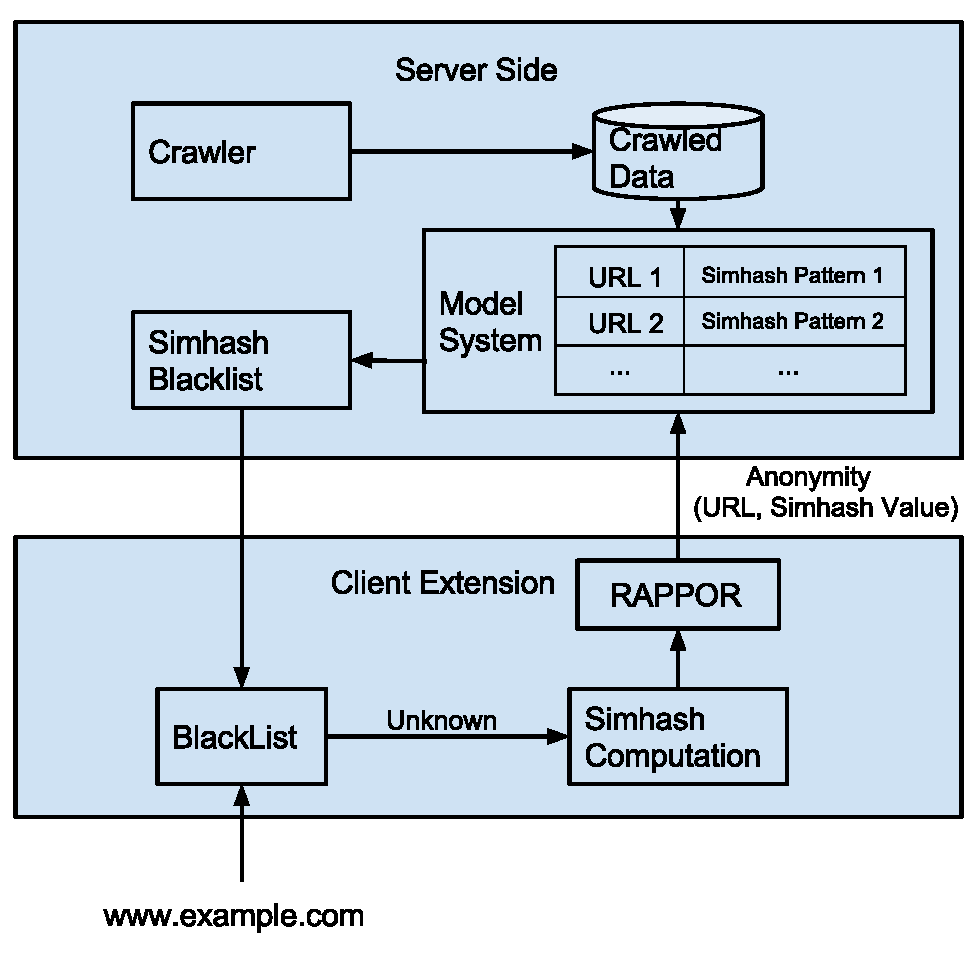
\includegraphics[width=.5\textwidth]{fig/crowdsourcing-cloaking-detection-system}
  \caption{Workflow of crowdsource cloaking detection sysetem}
  \label{fig:workflow}
\end{figure}

%The workflow ~\autoref{fig:workflow} is to collect page contents simhash on the user side, and compare
%them to simhash of the same link from ad serving company to find cloaking. When
%the differences of the simhashes are significantly large, the page is marked
%cloaking. We generate two simhash for page content and structure respectively.
%Intuition behind this is, simhash difference between different sites are larger
%than different visits of the same site. We build a two-phase system to detect
%cloaking: cluster learning phase, and cloaking detection phase. In the cluster
%learning phase, an ad company visit urls and generate simhash from its content
%with its owned IP, and learn pattern and distribution of the simhashes, i.e.
%simhash-based website model. In the cloaking detection phase, the ad company
%collects simhash from its users. Compare them with learned patterns, return
%cloaking score or mismatch
%
